%%%%%%%%%%%%%%%%%%%%%%%%%%%%%%%%%%%%%%%%%%%%%%%%%%%%%%%%%%%%%%%%%%%%%%%%%%%%%
\chapter{Implementation}
\label{chap:implementation}
%%%%%%%%%%%%%%%%%%%%%%%%%%%%%%%%%%%%%%%%%%%%%%%%%%%%%%%%%%%%%%%%%%%%%%%%%%%%%
\chapterstart

\section{Implementierung der Microservices} \label{sec:impl}
Kapitel \ref{sec:impl} fokussiert sich auf die Implementierung von Microservices, ein Kernaspekt für die Entwicklung skalierbarer Anwendungsarchitekturen. Abschnitt \ref{subsec:techstack} erläutert die Auswahl des Technologiestacks und bietet Einblicke in die Entscheidungsgrundlagen für die verwendeten Technologien. Der Prozess zur Entwicklung der Microservices wird in Abschnitt \ref{subsec:entwmicro} dargestellt, inklusive der methodischen Schritte zur Erstellung der Services. Abschnitt \ref{subsec:eventbas} diskutiert die Implementierung eventbasierter Kommunikation zwischen den Microservices.
\subsection{Auswahl und Begründung des Technologiestacks} \label{subsec:techstack}
Für die Entwicklung der Microservices wurde das Spring Framework in Kombination mit Java eingesetzt. Java, eine objektorientierte Programmiersprache, bildet die Grundlage für die Erstellung von stabilen und wartbaren Anwendungen. Die Wahl von Java stützt sich zudem auf dessen weitreichende Verbreitung, was für die Evaluierung der beiden Hypothesen relevant ist. Diese Entscheidung basiert auf den Erkenntnissen aus Umfragen, beispielweise \citetitle{pyp}~\parencite[vgl.][]{pyp}, das die Verbreitung von Programmiersprachen in der Softwareentwicklung thematisiert. Auch das Buch \citetitle{vitale}~\parencite[vgl.][]{vitale} nennt Programmiersprachen für Cloud-native Applikationen. Vor diesem Hintergrund wurde Java als objektorientierte Programmiersprache für das Projekt herangezogen. 

Das Spring-Framework spielt in diesem Werk eine zentrale Rolle bei der Entwicklung von Microservices mit Java, indem es wesentliche Funktionen für Dependency-Injection bietet. Insbesondere erleichtert es die Integration mit Technologien wie Datenbankverbindungen und die Anbindung an Message-Broker. Spring Boot, eine Erweiterung des Spring-Frameworks, vereinfacht zusätzlich die Softwareentwicklung in diesem Bereich. Die Umsetzung jedes Services erfolgt als Java/Spring Microservice, gemäß der in dieser Arbeit vorgenommenen Implementierungsentscheidung. Es ist jedoch zu beachten, dass Microservices, abhängig von der Architekturentscheidung, auch auf anderen Technologiestacks basieren können, sofern sie die definierten externen Schnittstellen beibehalten. Diese Flexibilität wurde bereits in Kapitel \ref{chap:concept} diskutiert.

\subsection{Entwicklungsprozess der Microservices} \label{subsec:entwmicro}
Zur Erstellung jedes Microservices dient Backstage, ein von Spotify entwickeltes Scaffolding Tool. Dieses Tool automatisiert den Erstellungsprozess von Projekten, indem es auf ein vordefiniertes Template\footnote{\url{https://github.com/avollmaier/templates}}, bekannt als Skeleton, zugreift und daraus eine Applikation generiert. Der Konfigurationsprozess für die Generierung sowie das Skeleton müssen nur einmal definiert werden, können jedoch für die Produktion weiterer Microservices beliebig oft repliziert werden. Das verwendete Skeleton bietet eine standardisierte Struktur, die die Einhaltung von Best Practices und konsistenten Entwicklungsstandards innerhalb der Microservice-Architektur sicherstellt.

Die Nutzung des Build-Tools ''Gradle'' im Projekt legt eine spezifische Projektstruktur fest, die eingehalten werden muss. Gradle strukturiert Projekte in einer Weise, die eine klare Trennung zwischen Produktionscode und Testcode fördert. Diese Strukturierung erleichtert die Build-Automatisierung und verbessert die Übersichtlichkeit des Projekts~\parencite[vgl.][]{gradledocs}{}. Das \lstinline{src}-Paket, das den Quellcode enthält, wird üblicherweise in Unterordner wie \lstinline{main} für den Anwendungscode und \lstinline{test} für den Testcode unterteilt. Die Verwendung von JUnit für die Testfälle im \lstinline{test}-Paket ermöglicht  eine standardisierte und weitverbreitete Methode für Unit-Tests in Java-Projekten, was die Qualitätssicherung der Software unterstützt.
\begin{figure}[H]
    \begin{center}
        \begin{forest}
            for tree={
            font=\ttfamily,
            grow'=0,
            child anchor=west,
            parent anchor=south,
            anchor=west,
            calign=first,
            edge path={
            \noexpand\path [draw, \forestoption{edge}]
            (!u.south west) +(7.5pt,0) |- node[fill,inner sep=1.25pt] {} (.child anchor)\forestoption{edge label};
            },
            before typesetting nodes={
            if n=1
            {insert before={[,phantom]}}
            {}
            },
            fit=band,
            before computing xy={l=15pt},
            }
            [<project-root>
            [src
            [main
            [java
            [resources]
            ]
            ]
            [test
            [java
            [resources]
            ]
            ]
            ]
            ]
        \end{forest}
    \end{center}
    \caption[Vorgegebene Standard Projektstruktur von Gradle]{Vorgegebene Standard Projektstruktur von Gradle~\parencite[vgl.][]{gradledocs}{}.}
\end{figure}

Im Rahmen der \ac{DDD} Strategie, welche für den Prototypen angewandt wird, erfolgt die Entwicklung der Microservices mit dem Ziel, Infrastruktur, Domäne und Applikationsschicht voneinander zu isolieren. Spring unterstützt diesen Prozess durch Bereitstellung spezifischer Tools für jede Schicht. Das Paket \lstinline{org.springframework.boot:spring-boot-starter-web} ermöglicht die Erstellung von Web-Anwendungen, die für die Handhabung von REST-Anfragen im Manager Service verwendet werden. Das Paket \lstinline{org.springframework.boot:spring-boot-starter-data-mongodb} dient zur Anbindung einer MongoDB an den Manager-Service. Diese Werkzeuge fördern die Umsetzung von \ac{DDD}, indem sie eine effiziente Strukturierung und Entkopplung der Systemkomponenten ermöglichen.

\begin{figure}[H]
    \centering
    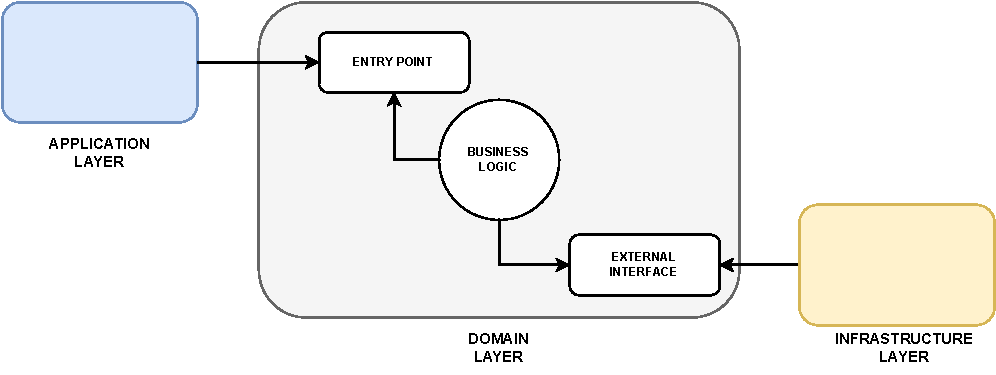
\includegraphics[width=14cm]{images/60_implementation/DDD.drawio.pdf}
    \caption[Darstellung des Domain-Driven-Designkonzepts]{Darstellung des Domain-Driven-Designkonzepts samt Visualisierung der Application-, Domain- und Infrastructure-Layer.}
    \label{fig:DDD}
\end{figure}
\newpage
Die vorliegende Grafik zeigt eine Projektstruktur, die sich an den Prinzipien des \ac{DDD} orientiert. Diese Struktur wird als Leitfaden für alle Implementierungen der Microservices genutzt, wobei die Abhängigkeiten zwischen den Paketen gemäß der in Abbildung \ref{fig:DDD} definierten Beziehungen festgelegt und implementiert werden. Innerhalb dieser Struktur sind verschiedene Pakete zu finden:

\begin{itemize}
    \item \textbf{config}: Dieses Paket enthält Konfigurationsdateien und -klassen, die für das Gesamtprojekt relevant sind, wie beispielsweise Datenbankverbindungen oder Sicherheitseinstellungen.
    
    \item \textbf{domain}: Der Kern des DDD-Ansatzes, das Domain-Paket, beherbergt die Geschäftslogik und ist unterteilt in:
    \begin{itemize}
        \item \textbf{exception}: Klassen, die spezifische Ausnahmen und Fehlerbehandlungen für die Domäne definieren.
        \item \textbf{model}: Enthält die Domänenmodelle oder Entitäten.
        \item \textbf{repository}: Interfaces, die den Zugriff auf die Datenquelle abstrahieren, was für die Anbindung an Datenbanken im Sinne des Repository-Musters steht.
        \item \textbf{service}: Dienste, die Geschäftslogik-Operationen ausführen, indem sie auf Modelle und Repositories zugreifen.
    \end{itemize}
    
    \item \textbf{web}: Dieses Paket ist für die Präsentations- und Interaktionsschicht zuständig, welche die DDD-Schichten ergänzt:
    \begin{itemize}
        \item \textbf{controller}: Controller-Klassen, die eingehende HTTP-Anfragen verarbeiten und die entsprechenden Dienste der Applikationsschicht aufrufen.
        \item \textbf{dto}: Data-Transfer-Objects, die für die Übertragung von Daten zwischen Prozessen genutzt werden, oft als Teil des Controllers, um Daten in einem netzwerkfähigen Format zu senden oder zu empfangen.
    \end{itemize}
    
    \item \textbf{resources}: Ein Paket, das nicht standardmäßig im DDD-Konzept enthalten ist, jedoch häufig Ressourcen wie statische Inhalte, Vorlagen oder Konfigurationsdateien enthält.
\end{itemize}
\begin{figure}[H]
    \begin{center}
        \begin{forest}
            for tree={
            font=\ttfamily,
            grow'=0,
            child anchor=west,
            parent anchor=south,
            anchor=west,
            calign=first,
            edge path={
            \noexpand\path [draw, \forestoption{edge}]
            (!u.south west) +(7.5pt,0) |- node[fill,inner sep=1.25pt] {} (.child anchor)\forestoption{edge label};
            },
            before typesetting nodes={
            if n=1
            {insert before={[,phantom]}}
            {}
            },
            fit=band,
            before computing xy={l=15pt},
            }
            [<package root>
            [config]
            [domain
            [exception]
            [model]
            [repository]
            [service]
            ]
            [web
            [controller]
            [dto]
            ]
            [resources]
            ]
            ]
        \end{forest}
    \end{center}
    \caption{Gewählte Projektstruktur zur Aufteilung der Komponenten nach \acl{DDD}}
\end{figure}
Diese Strukturierung ermöglicht es, die Prinzipien des Domain-Driven-Designs umzusetzen, indem eine klare Trennung zwischen der Geschäftslogik (Domain), der Datenzugriffsschicht (Repositories), der Anwendungsschicht (Services) und der Präsentationsschicht (Web) etabliert wird.
\subsection{Realisierung der eventbasierten Kommunikation zwischen Microservices} \label{subsec:eventbas}
Die Interaktion zwischen den Microservices des Prototypen erfolgt über ein eventbasiertes Modell, implementiert durch das Framework Spring Cloud Stream. Spring Cloud Stream agiert als abstrahierende Schicht, die eine einheitliche Schnittstelle zur Anbindung verschiedener Messaging-Systeme bietet~\parencite[vgl.][]{springcloudstream}. Diese Abstraktion erlaubt es Entwickler/innen, unabhängig vom spezifischen Typ des Messaging-Systems, eine Kommunikation zwischen den Message-Broker und Applikation zu realisieren.

Die Integration von Spring Cloud Stream in einen Microservice des Prototypen erfordert die entsprechende Konfiguration im \lstinline{build.gradle}-File des jeweiligen Projekts. Die Konfiguration der Abhängigkeiten ist in \ref{lst:config1} zu sehen.
\newpage

 \lstinputlisting[language=Java,
                   aboveskip=\floatsep,
                   belowskip=\floatsep,
                   xleftmargin=0cm,         % no extra margins for floats
                   xrightmargin=0cm,        % no extra margins for floats
                   label=lst:config1,   % reference to this listing
                   firstline=22,            % include just a few lines 
                   lastline=26,             % of the given file
                   caption={Konfiguration der notwendigen Spring Cloud Stream Abhängigkeiten.}
                  ]{src/build.gradle}         % the file to be included


Spring Cloud Stream unterstützt eine Vielzahl von Binder-Implementierungen, die für die Integration mit externen Messaging-Systemen konzipiert sind \parencite[vgl.][]{springcloudstream}. Diese Implementierungen umfassen drei zentrale Komponenten: \textit{Destination Binders}, \textit{Destination Bindings} und \textit{Messages}. In den folgenden Abschnitten werden diese erläutert. Zudem wird explizit auf die Konfiguration eingegangen, da diese die essentiellen Bausteine für die Kommunikation der Services sind.
\begin{enumerate}
  \item \textbf{Destination Binder}: Dient als Schnittstelle zwischen den Spring Cloud Stream Anwendungen und dem externen Messaging-System und ist verantwortlich für die Konfiguration der Verbindung.
  \item \textbf{Destination Bindings}: Repräsentieren die Verknüpfung zwischen der Anwendungslogik und den Nachrichtenkanälen des Messaging-Systems.
  \item \textbf{Messages}: Stellen die grundlegende Einheit der Kommunikation dar, die über die definierten Bindings ausgetauscht wird.
\end{enumerate}

\textbf{Konfiguration des Destination Binders}\newline
Die Konfiguration eines externen Messaging-Systems erfordert die spezifische Anpassung des \textit{Destination Binders}, abhängig von den Anforderungen des jeweiligen Systems und den Eigenschaften der Binder. Die Konfiguration dieses Destination Binders erfolgt mit einer Konfiguration (siehe Listing \ref{lst:config2}) des \textit{application.yml} Files im jeweiligen Microservice.
\newpage
 \lstinputlisting[language=Java,
                   aboveskip=\floatsep,
                   belowskip=\floatsep,
                   xleftmargin=0cm,         % no extra margins for floats
                   xrightmargin=0cm,        % no extra margins for floats
                   label=lst:config2,   % reference to this listing
                   firstline=76,            % include just a few lines 
                   lastline=84,             % of the given file
                   caption={[Spring Cloud Stream Konfiguration Destination Binder]Konfiguration des Destination Binders in der application.yml Datei für die Spring Cloud Stream Anbindung.}
                  ]{src/application.yml}         % the file to be included
\textbf{Konfiguration des Destination Bindings}\newline
Als nächsten Schritt muss eine Konfiguration des \textit{Destination Bindings} erfolgen. Dieses Binding verknüpft, wie bereits erwähnt, den Programmcode mit dem Messaging-System. 

Innerhalb der \textit{Destination Bindings} von Spring Cloud Stream wird eine Unterscheidung zwischen zwei Typen getroffen: Ausgehende Bindings, die Nachrichten an ein sogenanntes ''TopicExchange'' im Message-Broker senden (beispielweise \textbf{prioritize-out-0}), und eingehende Bindings, die eingehende Nachrichten mit dem eigentlichen Programmcode verbinden (beispielweise \textbf{prioritize-in-0}). Zu sehen ist diese Konfiguration in Listing \ref{lst:config3}.

\lstinputlisting[language=Java,
                   aboveskip=\floatsep,
                   belowskip=\floatsep,
                   xleftmargin=0cm,         % no extra margins for floats
                   xrightmargin=0cm,        % no extra margins for floats
                   label=lst:config3,   % reference to this listing
                   firstline=66,            % include just a few lines 
                   lastline=76,             % of the given file
                   caption={[Spring Cloud Stream Konfiguration Destination Bindings]Konfiguration des Destination Bindings in der application.yml Datei für die Definition der Input- und Output-Bindings}
                  ]{src/application.yml}         % the file to be included

Die \textit{Destination Bindings} innerhalb von Spring Cloud Stream weisen eine einheitliche Benennungskonvention auf, die eine logische Zuweisung und Identifikation innerhalb der Architektur in der Anwendung unterstützt. Durch die abstrakte Repräsentation der Applikation in Kombination mit dem verwendeten Messaging-Broker, erleichtert Spring Cloud Stream die Verwaltung und Konfiguration dieser Bindings. Die Spezifizierung von \lstinline{<functionName>} in der Konfiguration definiert explizit, welche Komponente der Applikation Nachrichten empfängt oder sendet. Der \lstinline{<index>} hingegen ist in diesem Kontext bei einer einzigen Input-Funktion standardmäßig auf 0 gesetzt.

\begin{itemize}
    \item \textbf{Input-Binding:} \lstinline{<functionName>} + \lstinline{-in-} + \lstinline{<index>}
        \item \textbf{Output-Binding:} \lstinline{<functionName>} + \lstinline{-out-} + \lstinline{<index>}
\end{itemize}
                  
Neben den Input- und Output-Bindings wird in Spring Cloud Stream auch eine \textit{Group}, bekannt als \textit{Consumer Group}, definiert. Diese ermöglicht die Bildung von Gruppen für Subscriber, die am selben Topic teilnehmen. Consumer Groups spielen eine zentrale Rolle bei der Skalierung und Nachrichtenverwaltung in verteilten Systemen, indem sie sicherstellen, dass Nachrichten an Topics nur einmal von einem Mitglied der Gruppe verarbeitet werden. Dieses Konzept wird durch den folgenden Auszug von \citeauthor{springcloudstream}~\parencite[vgl.][]{springcloudstream} verdeutlicht:

\begin{spar}
    \textit{While the publish-subscribe model makes it easy to connect applications through shared topics, the ability to scale up by creating multiple instances of a given application is equally important. When doing so, different instances of an application are placed in a competing consumer relationship, where only one of the instances is expected to handle a given message.~\parencite[][]{springcloudstream}}
\end{spar}

Die Festlegung der \textit{group}-Eigenschaft ist essentiell, wenn mehrere Instanzen eines Microservices bzw. Consumers vorhanden sind. Ohne die Spezifizierung einer \textit{Consumer Group} durch das \textit{group} Property würden alle Instanzen desselben Microservices identische Nachrichten vom Message-Broker empfangen. Die Konfiguration der \textit{group}-Eigenschaft stellt sicher, dass eine Nachricht nur von einer einzigen Instanz innerhalb der spezifizierten Gruppe verarbeitet wird, was der intendierten Funktionsweise entspricht.\newline

\textbf{Konfiguration der Nachricht für Input-/Output-Binding}\newline
Am Ende des Konfigurationsprozesses steht die Definition einer Nachricht, die über den Message-Broker an das entsprechende Topic gesendet wird. In diesem Szenario wird die Nachricht als einfacher Java-Record definiert, wie im Listing \ref{lst:pojo} dargestellt.
\newline
\lstinputlisting[language=Java,
                 xleftmargin=0cm,         % keine zusätzlichen Ränder für Floats
                 xrightmargin=0cm,        % keine zusätzlichen Ränder für Floats
                 label=lst:pojo,   % Referenz auf dieses Listing
                 firstline=7,             % nur einige Zeilen des angegebenen Files einbeziehen
                 lastline=7,              % des angegebenen Files
                 caption={[Java-Record Message Definition]       % Kurzer Titel für das Listingverzeichnis
                           Implementierung eines 
                           Java-Records für eine zu sendende Nachricht über eine StreamBridge Instanz.}
                ]{src/AddressSuppliedMessage.java}

\textbf{Publish einer Nachricht über das Output-Binding}\newline
Anschließend wird die definierte Nachricht mittels der \textit{Stream Bridge} adressiert, einem von Spring Cloud Stream bereitgestellten Bean. Die \textit{Stream Bridge} ermöglicht das Publizieren der vordefinierten Nachricht an den Message-Broker. Das nachfolgende Listing \ref{lst:streambridge} illustriert die Nutzung der injizierten \textit{Stream Bridge} innerhalb einer Methode der Service-Komponente des Manager-Microservices.


\begin{lstlisting}[language=Java, caption=Beispiel einer Methode zur Verarbeitung ausgehender Nachrichten., label={lst:streambridge}]
private final CrawlerManagerRepository crawlerManagerRepository;
private final StreamBridge streamBridge;

public CrawlerManagerService(CrawlerManagerRepository crawlerManagerRepository, StreamBridge streamBridge) {
    this.crawlerManagerRepository = crawlerManagerRepository;
    this.streamBridge = streamBridge;
}
...
private void publishAddressSupplyEvent(Crawler crawler) {
    //UUID zur identifikation der Crawler Konfiguration
    UUID crawlerId = crawler.id();
    
    List<URL> publishAddresses = identifyPublishAdresses(crawler);

    //Erstellen der Message
    var addressSupplyMessage = new AddressSuppliedMessage(crawlerId, publishAddresses);

    //SUPPLY_ADDRESS_OUT = "supplyAddress-out-0"
    var result = streamBridge.send(SUPPLY_ADDRESS_OUT, addressSupplyMessage);
    ...
\end{lstlisting}
\textbf{Subscriben eines Topics über das Input-Binding}\newline
Nach der Konfiguration des Input-Bindings können eingehende Nachrichten durch eine mit \textit{@StreamListener} annotierte Methode (siehe \ref{lst:processIncom}) oder durch die Verwendung von funktionalen Programmiermodellen in Spring Cloud Stream verarbeitet werden. Diese Methoden werden automatisch aufgerufen, wenn eine neue Nachricht im abonnierten Topic erscheint, wodurch die asynchrone Verarbeitung von Ereignissen innerhalb des Microservices ermöglicht wird.
\newpage
\begin{lstlisting}[language=Java, caption=Beispiel einer Methode zur Verarbeitung eingehender Nachrichten., label={lst:processIncom}]
@StreamListener(target = "input")
public void processIncomingMessage(String message) {
    // Logik zur Verarbeitung der Nachricht
}
\end{lstlisting}


Durch den Einsatz von Spring Cloud Stream wird die Verbindung jedes Microservices mit dem Message-Broker ermöglicht, was zu einer  asynchronen Kommunikationsfähigkeit zwischen den Services führt. Diese Architektur ermöglicht es den Microservices, unabhängig voneinander zu operieren und gleichzeitig miteinander zu kommunizieren. Die asynchrone Natur der Kommunikation erleichtert die Skalierung unter hohen Lastbedingungen, indem zusätzliche Instanzen dynamisch hinzugefügt werden können, um die Rechenlast zu verteilen. Diese neuen Instanzen ziehen Nachrichten aus der Queue und verarbeiten sie, wodurch die Gesamtleistung des Systems bei Bedarf flexibel angepasst werden kann. Mit dieser Implementierung wurde unter anderem die Basis für die Evaluierung (Kapitel \ref{sec:comparisonmicroservice}) geschaffen.

\section{Optimierung durch \acl{AOT}} \label{sec:aotoptimizing}
Das Kapitel \ref{sec:aotoptimizing} thematisiert die Optimierung des Prototypen durch \acl{AOT}, welche die Ausführungseffizienz und Startzeit von Anwendungen verbessert. Strategien zur Integration der \acl{AOT} werden in Abschnitt \ref{subsec:trasformationtoaot} vorgestellt. Die Umwandlung des Prototypen in native Images wird in Abschnitt \ref{subsec:integrationaot} beschrieben.
\subsection{Strategien zur Integration der \acl{AOT}} \label{subsec:trasformationtoaot}
Spring Native bietet einen Mechanismus zur Kompilierung von Spring Boot Anwendungen durch GraalVM, mit dem Ziel, jede Spring-Applikation in eine nativ ausführbare GraalVM-Applikation zu transformieren. Dieser Prozess zielt darauf ab, ohne Modifikationen am bestehenden Applikationscode durchführbar zu sein. Dies wird durch die offizielle Dokumentation von \citeauthor{springnative}~\parencite[vgl.][]{springnative}{} unterstrichen.

Die Realisierung dieses Ziels wird durch die Nutzung von Gradle oder Maven-Plugins erleichtert, die alle notwendigen Konfigurationen für die \ac{AOT} der Spring-Klassen durch den GraalVM-Native-Compiler enthalten. Die spezifische Anwendung dieser Plugins und die damit verbundene Konfiguration werden im Kapitel \ref{subsec:integrationaot} detailliert beschrieben.

Um eine Spring Boot Jar in nativen Code zu konvertieren, stehen zwei verschiedene Strategien zur Verfügung. Die erste Methode nutzt das von GraalVM bereitgestellte Command-Line-Tool \lstinline{native-image}, um ein natives Image zu erstellen. Der Befehl hierfür lautet: \lstinline{native-image [options] -jar jarfile [imagename] [options]}. Eine Voraussetzung für die Erstellung eines nativen Images ist das Vorhandensein eines Jar-Archivs oder einer \lstinline{class}-Datei.

Eine alternative Methode zur Erstellung eines \ac{AOT}-Images bietet der Einsatz von Buildpacks, welcher im folgenden Kapitel \ref{subsec:integrationaot} eingehender betrachtet wird, da diese Kompilierungsvariante im Prototypen Anwendung findet.

\subsection{Integration mittels Buildpacks} \label{subsec:integrationaot}
Die Kompilierung einer ausführbaren JAR in ein natives Image mittels Buildpacks\footnote{\url{https://buildpacks.io/}}, insbesondere durch deren Implementierung Paketo\footnote{\url{https://paketo.io/}}, bietet eine standardisierte Methode zur Erstellung von Cloud-nativen Images. Der Buildpacks-Standard zielt darauf ab, die Kompilierung von Cloud-nativen Images zu vereinheitlichen und zu vereinfachen.

Die Kompilierung eines nativen Images mittels Buildpacks erfolgt durch das Command-Line-Tool von Paketo, ''pack''. Dieses Werkzeug ermöglicht eine Erstellung von nativen Images. Der Einsatz von `pack` zur Generierung eines nativen Images wird durch den folgenden Befehl in Listing \ref{lst:bpnative} realisiert.

\begin{lstlisting}[language=bash, caption={Erstellung eines nativen Images mit dem Command-Line-Tool ''pack''.},label={lst:bpnative}]
pack build --builder paketobuildpacks/builder-jammy-tiny \
    --path <path-to-application-jar> \
    --env 'BP_NATIVE_IMAGE=true' \
    service:0.0.1-SNAPSHOT
\end{lstlisting}

Die Ausführung des oben genannten ''pack''-Befehls resultiert in der Erstellung eines nativen Images, das als Container Image exportiert wird. Dieses Image lässt sich in einer Docker-Umgebung mit dem Befehl \lstinline{docker run} starten. Zu sehen ist das in Listing \ref{lst:dockerrun}.

\begin{lstlisting}[language=bash, caption={Starten des nativen Images als Docker-Container.}, label={lst:dockerrun}]
docker run --rm -p 8080:8080 docker.io/library/service:0.0.1-SNAPSHOT
\end{lstlisting}

Um die Erstellung von AOT-Images zu unterstützen, wurde in der \lstinline{build.gradle}-Datei jedes Services ein spezifischer Task mittels Groovy hinzugefügt. Dieser Task ist für das Setzen umgebungsspezifischer Konfigurationen verantwortlich, analog zu den im obigen Befehl dargestellten Einstellungen. Die Integration dieses Schritts in den Buildprozess vereinfacht die Handhabung und Konfiguration der AOT-Kompilierung. Der folgende Groovy-Code (siehe Listing \ref{lst:bootbuildimage}) illustriert die Implementierung eines solchen Tasks im Buildprozess.

\begin{lstlisting}[language=Java, caption={Gradle Task für die Erstellung eines Docker Images mit Paketo Buildpacks.},label={lst:bootbuildimage}]
...
tasks.named('bootBuildImage') {
    builder = 'paketobuildpacks/builder:base'

    if(System.getenv('NATIVE_IMAGE_ENABLED') == 'enabled'){
        println("bootBuildImage is building a native image")
        environment = ['BP_NATIVE_IMAGE': 'true']
    } else {
        environment = ['BP_LIVE_RELOAD_ENABLED': 'true']
    }

    imageName = "${project.name}"

    docker {
        publishRegistry {
            username = project.findProperty("registryUsername")
            password = project.findProperty("registryToken")
            url = project.findProperty("registryUrl")
        }
    }
}
...
\end{lstlisting}
In der gezeigten \lstinline{build.gradle}-Datei (siehe Listing \ref{lst:bootbuildimage}) ist die Konfiguration des Gradle-Tasks (\lstinline{bootBuildImage}) dargestellt, welcher das Paketo Buildpack für die Erstellung eines Docker Images verwendet. Dieser Task wählt basierend auf der Umgebungsvariable \lstinline{NATIVE_IMAGE_ENABLED} zwischen der Erstellung eines nativen Images und der Aktivierung des Live-Reloads. Zudem wird der Image-Name auf den Projektnamen gesetzt und, falls vorhanden, das Docker Image in ein spezifiziertes Docker-Registry hochgeladen.
\chapterend